%% main.tex
%% Copyright 2021 Paulo Henrique De Moura
%
% This work may be distributed and/or modified under the
% conditions of the LaTeX Project Public License, either version 1.3
% of this license or (at your option) any later version.
% The latest version of this license is in
%   http://www.latex-project.org/lppl.txt
% and version 1.3 or later is part of all distributions of LaTeX
% version 2005/12/01 or later.
%
% This work has the LPPL maintenance status `maintained'.
%
% The Current Maintainer of this work is Paulo Henrique De Moura
%
% This work consists of the files ifgw.cls and main.tex
%% Copyright 2005 Paulo Henrique De Moura
%
% This work may be distributed and/or modified under the
% conditions of the LaTeX Project Public License, either version 1.3
% of this license or (at your option) any later version.
% The latest version of this license is in
%   http://www.latex-project.org/lppl.txt
% and version 1.3 or later is part of all distributions of LaTeX
% version 2005/12/01 or later.
%
% This work has the LPPL maintenance status `maintained'.
%
% The Current Maintainer of this work is Paulo Henrique De Moura.
%
% This work consists of the files ifgw.cls and main.tex.
%
\documentclass{ifgw}
\usepackage{amsmath}
\usepackage{cite}
\usepackage{fourier}
\usepackage{lipsum}
\usepackage{pdfpages}

\author{Anakin Skywalker}
\city{Tatooine}
\cosupervisor[Coorientador]{Obi-Wan Kenobi}
\logo[align=left]{Images/unicamp.png}
\supervisor[Orientador]{Master Yoda}

\title{
    english={Star Wars},
    portuguese={Guerra nas estrelas},
}

\subtitle{
    english={May the Force be with you},
    portuguese={Que a Força esteja com você},
}

\institute{
    english={Darth Plagueis Institute},
    portuguese={Instituto Darth Plagueis},
}

\university{
    english={University of the Galactic Empire},
    portuguese={Universidade do Império Galático},
}

\backcover{
    portuguese declaration={
        Tese apresentada ao \theinstitute~da \theuniversity~como
        parte dos requisitos exigidos para a obtenção do título de
        \uppercase{Doutor em Ciências}, na Área de \uppercase{Física}.
    },
    english declaration={
        Thesis presented to the \theinstitute[e]~of the \theuniversity[e]~in
        partial fulfillment of the requirements for the de\-gree of
        \uppercase{Doctor of Science}, in the area of \uppercase{Physics}.
    },
    version={
        Es\-te tra\-ba\-lho cor\-res\-pon\-de à ver\-são fi\-nal da
        te\-se de\-fen\-di\-da pe\-lo a\-lu\-no \theauthor~e
        ori\-en\-ta\-da pe\-lo Prof. Dr. \thesupervisor.
    },
    language=portuguese,
}

\begin{document}

\maketitle
\makebackcover

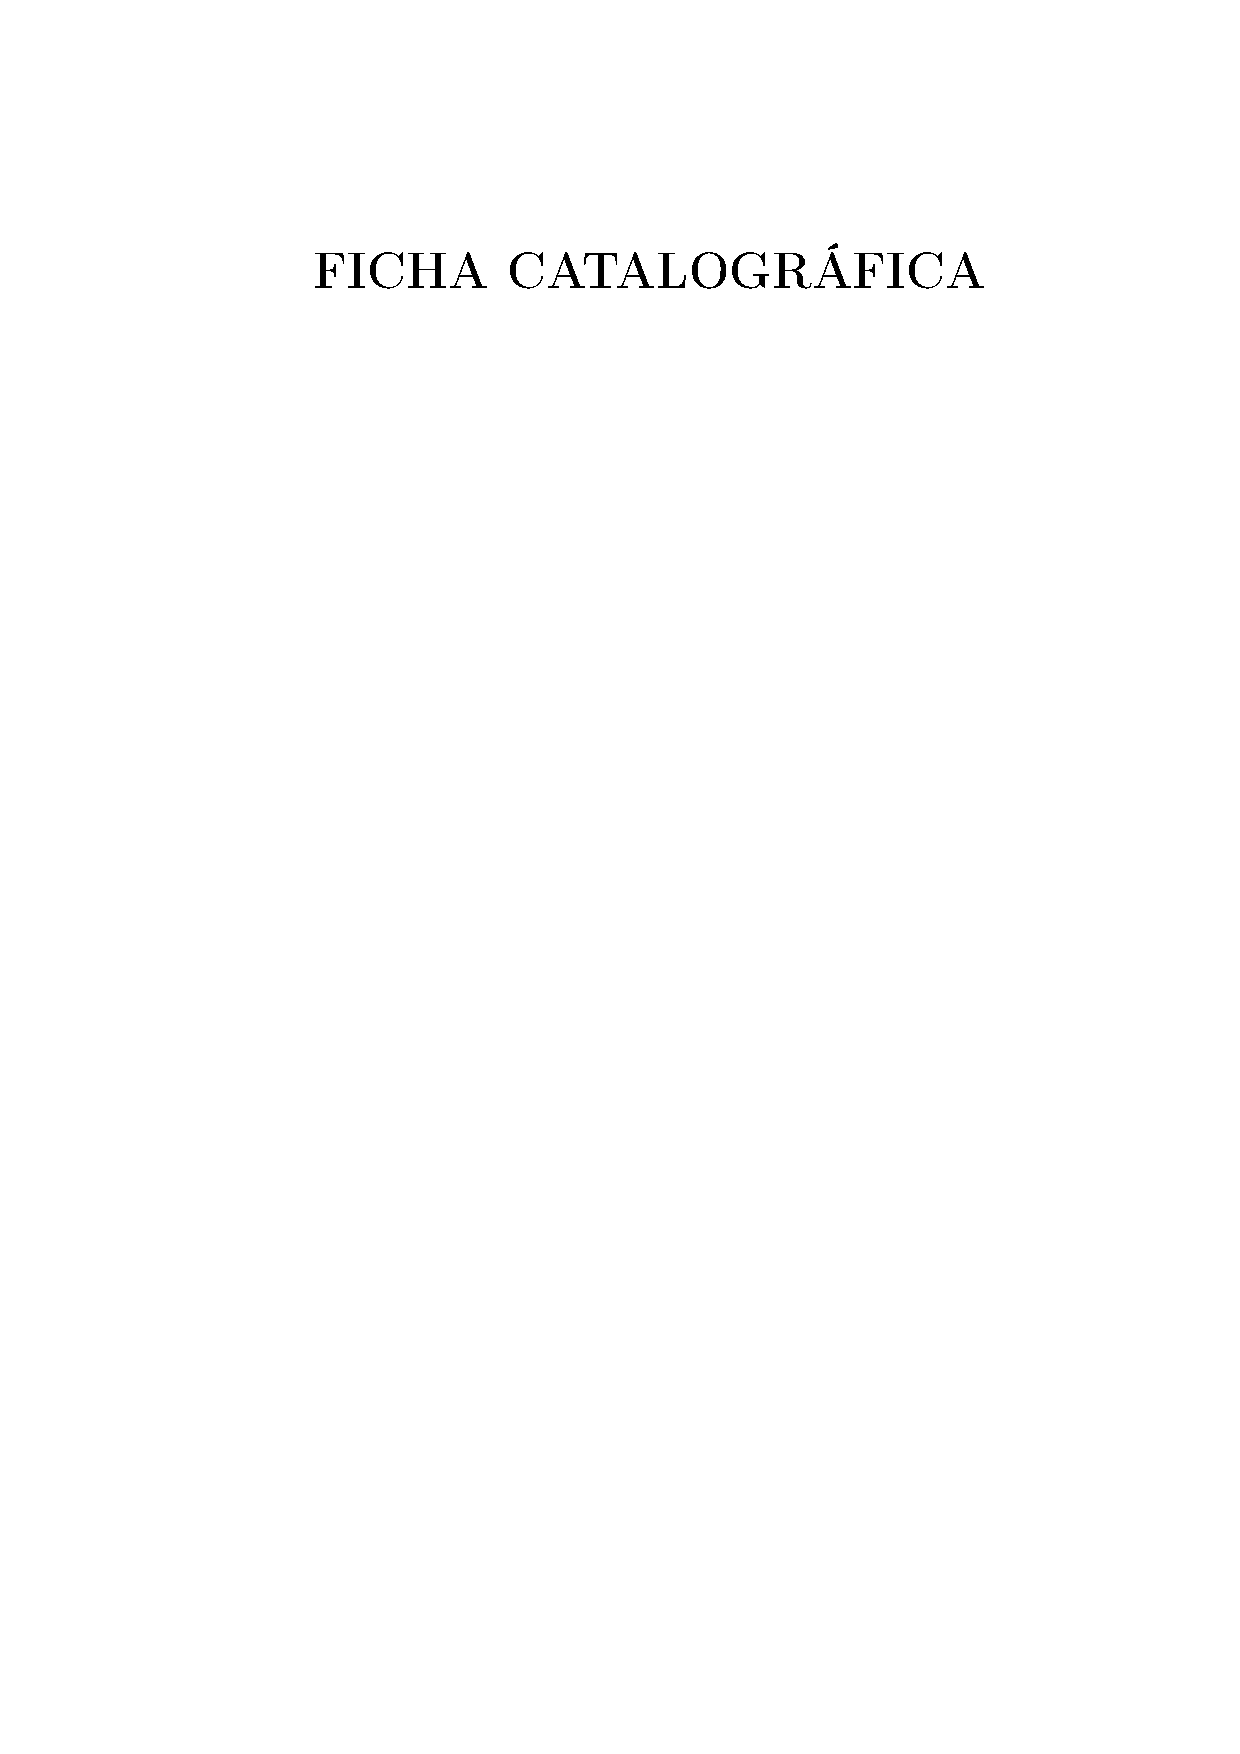
\includepdf[pages=-]{PDFs/ficha_catalografica}
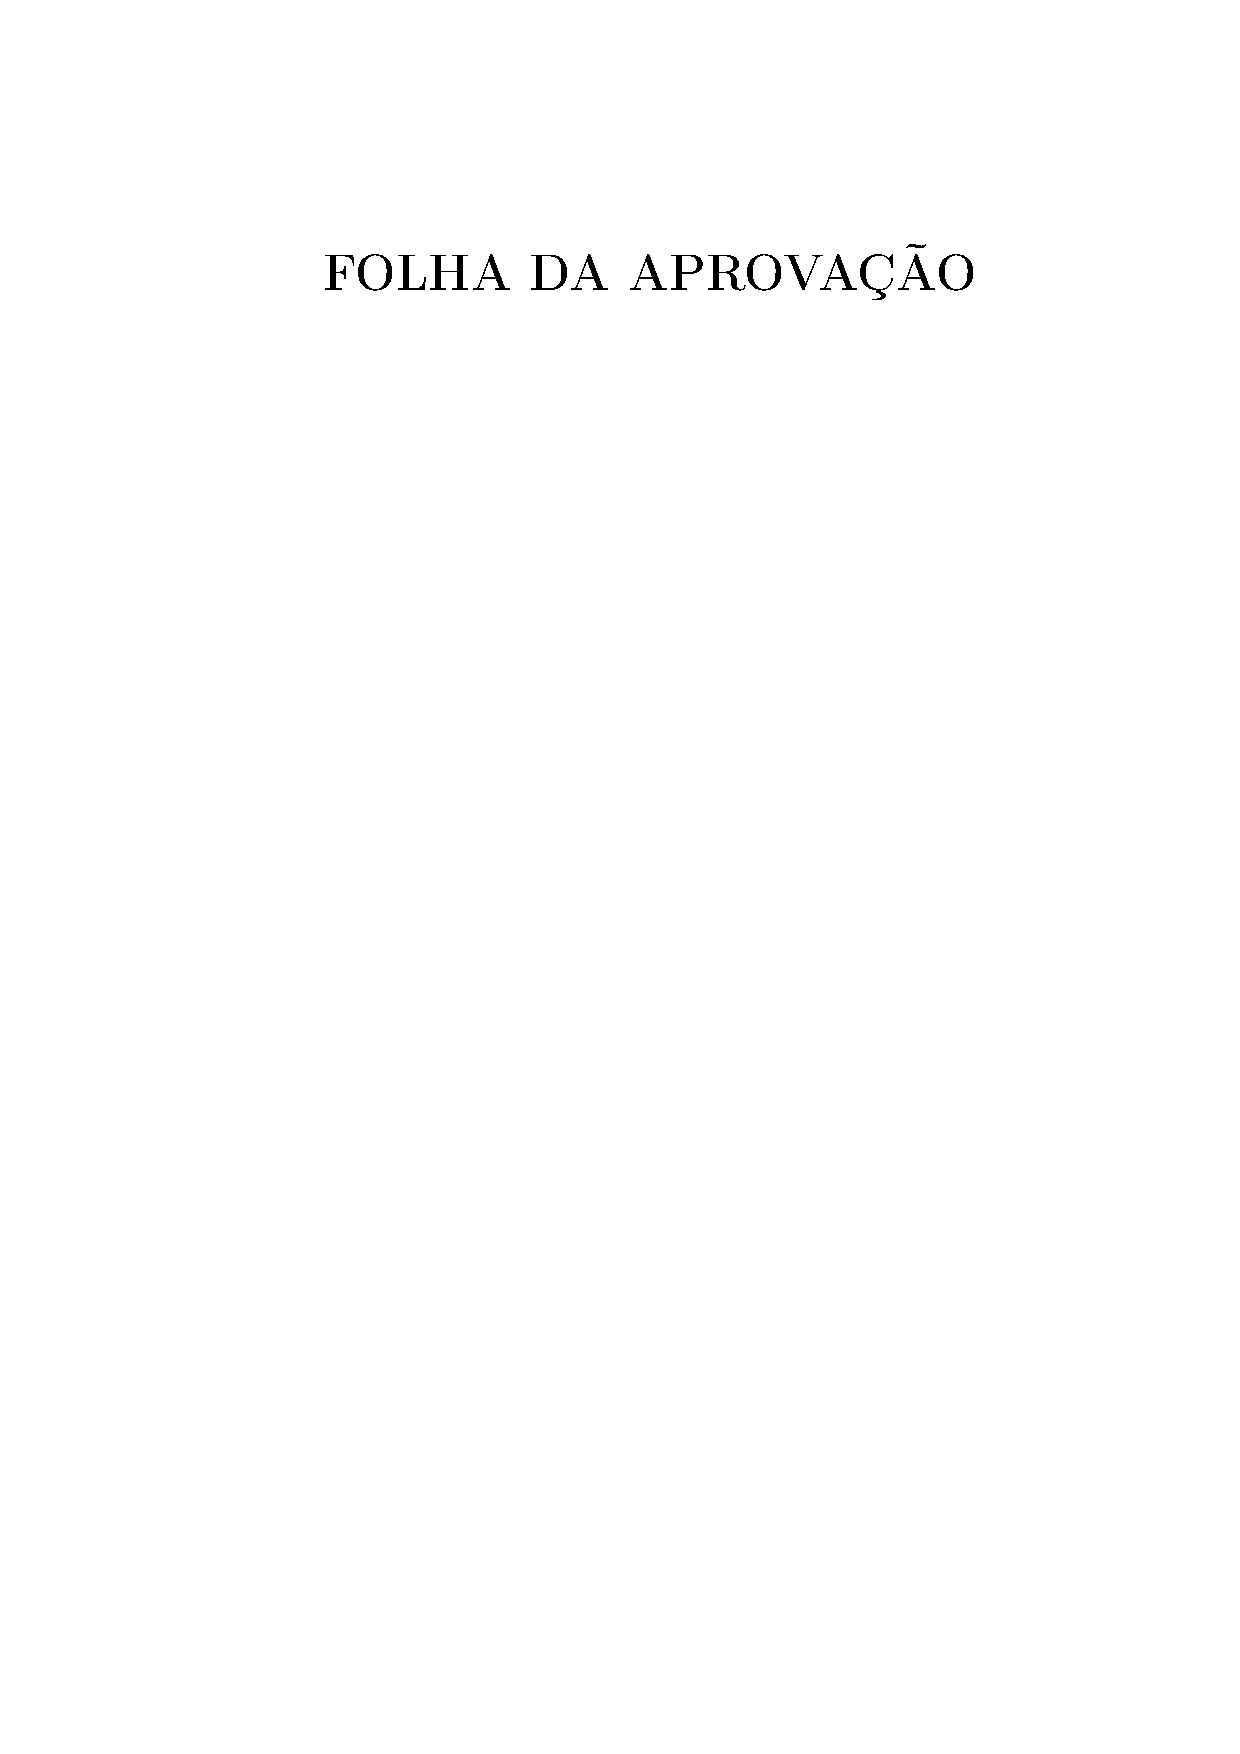
\includepdf[pages=-]{PDFs/folha_de_aprovacao}

\dedication{To my son, Luke Skywalker.}
\epigraph{Master Yoda}{May the Force be with you!}

\begin{abstract}[name=Acknowledgements]
\lipsum[1]
\end{abstract}

\begin{abstract}[name=Resumo]
\lipsum[1]
\end{abstract}

\begin{abstract}
\lipsum[1]

\begin{equation}
\braket[H]{\alpha}{\beta}
\end{equation}

\begin{equation}
\braket{\alpha}{\beta}
\end{equation}

\begin{equation}
\braket[]{\alpha}{\beta}
\end{equation}

\end{abstract}


\listoffigures
\listoftables
\tableofcontents

\chapter{A New Hope}
\section{It is a period of civil war}
Rebel spaceships, striking from a hidden base, have won 
their first victory against the evil Galactic Empire.  
During the battle, Rebel spies managed to steal secret 
plans to the Empire's ultimate weapon, the DEATH STAR, 
an armored space station with enough power to destroy 
an entire planet. Pursued by the Empire's sinister 
agents, Princess Leia races home aboard her starship, 
custodian of the stolen plans that can save her people 
and restore freedom to the galaxy.

\lipsum[1-3]
\cite{CHAUDHURI_2014,MATSUI_1986,MROWCZYNSKI_1998}

\begin{center}
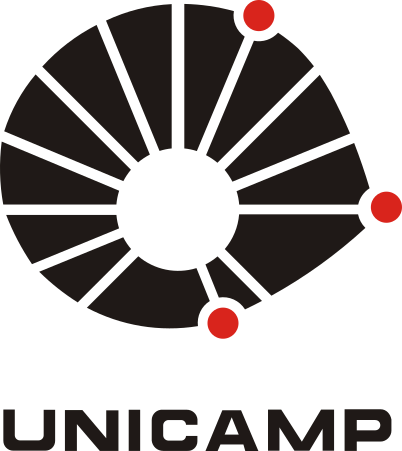
\includegraphics[width=.35\textwidth]{Images/unicamp.png}
\captionof{figure}{\lipsum[12]}
\end{center}

\lipsum[4-10]

\ncc

\begin{equation}
\njp
\end{equation}

\begin{equation}
\kdelta
\end{equation}

\chapter{The Empire Strikes Back}
\section{It is a dark time for the Rebellion}
 
Although the Death Star has been destroyed, Imperial troops 
have driven the Rebel forces from their hidden base and 
pursued them across the galaxy.  Evading the dreaded 
Imperial Starfleet, a group of freedom fighters led by Luke 
Skywalker has established a new secret base on the remote 
ice world of Hoth.  The evil lord Darth Vader, obsessed with 
finding young Skywalker, has dispatched thousands of remote 
probes into the far reaches of space.
\begin{equation}
\njp \sim \frac{\Ncoll \cxjp}{\cxnn}
\end{equation}
\lipsum[1-10]
\cite{THEWS_2001}
\cite{FLORKOWSKI_2010}
\cite{GROSS_1973}

\Npart

\chapter{Return of the Jedi}
Luke Skywalker has returned to his home planet of Tatooine 
in an attempt to rescue his friend Han Solo from the 
clutches of the vile gangster Jabba the Hutt.  Little does 
Luke know that the GALACTIC EMPIRE has secretly begun 
construction on a new armored space station even more 
powerful than the first dreaded Death Star.  When completed, 
this ultimate weapon will spell certain doom for the small 
band of rebels struggling to restore freedom to the galaxy \cite{bib_hutt83, bib_solo83, bib_skywalker83, bib_boba83}.

\lipsum[1-10]

\chapter{The Phantom Menace	May}
\section{Turmoil has engulfed the Galactic Republic}
The taxation of trade routes to outlying star systems is in 
dispute. Hoping to resolve the matter with a blockade of 
deadly battleships, the greedy Trade Federation has stopped 
all shipping to the small planet of Naboo. While the Congress 
of the Republic endlessly debates this alarming chain of 
events, the Supreme Chancellor has secretly dispatched two 
Jedi Knights, the guardians of peace and justice in the 
galaxy, to settle the conflict \cite{bib_binks99, bib_quigon99}.

\lipsum[1-10]

\chapter{Attack of the Clones}	
\section{There is unrest in the Galactic Senate}
Several thousand solar systems have declared their intentions 
to leave the Republic. This separatist movement, under the 
leadership of the mysterious Count Dooku, has made it 
difficult for the limited number of Jedi Knights to maintain 
peace and order in the galaxy. Senator Amidala, the former 
Queen of Naboo, is returning to the Galactic Senate to vote 
on the critical issue of creating an ARMY OF THE REPUBLIC to 
assist the overwhelmed Jedi \cite{bib_amidala02, bib_palpatine02, bib_jarjar02, bib_anakin02, bib_dooku02}.

\lipsum[1-10]

\chapter{Revenge of the Sith}	
\section{War!}
The Republic is crumbling under attacks by the ruthless Sith 
Lord, Count Dooku. There are heroes on both sides. Evil is 
everywhere. In a stunning move, the fiendish droid leader, 
General Grievous, has swept into the Republic capital and 
kidnapped Chancellor Palpatine, leader of the Galactic Senate. 
As the Separatist Droid Army attempts to flee the besieged 
capital with their valuable hostage, two Jedi Knights lead 
a desperate mission to rescue the captive Chancellor.

\lipsum[1-10]
\cite{THEWS_2001}


\bibliographystyle{naturemag}
\bibliography{Chapters/Bibliografia}

\appendix
\chapter{The Force Awakens}
\section{Luke Skywalker has vanished}
In his absence, the sinister FIRST ORDER has risen from the 
ashes of the Empire and will not rest until Skywalker, the 
last Jedi, has been destroyed. With the support of the 
REPUBLIC, General Leia Organa leads a brave RESISTANCE. She 
is desperate to find her brother Luke and gain his help in 
restoring peace and justice to the galaxy. Leia has sent her 
most daring pilot on a secret mission to Jakku, where an old 
ally has discovered a clue to Luke's whereabouts \cite{bib_snoke15}.

\lipsum[1-10]

\chapter{The Last Jedi}
\section{The FIRST ORDER reigns}
Having decimated the peaceful Republic, Supreme Leader Snoke 
now deploys his merciless legions to seize military control 
of the galaxy. Only General Leia Organa's band of RESISTANCE 
fighters stand against the rising tyranny, certain that Jedi 
Master Luke Skywalker will return and restore a spark of hope 
to the fight. But the Resistance has been exposed. As the 
First Order speeds toward the rebel base, the brave heroes 
mount a desperate escape \cite{bib_chirrut17, bib_rey17}.

\lipsum[1-10]

\chapter{The Rise of Skywalker}
\section{The dead speak!}
The galaxy has heard a mysterious broadcast, a threat of 
REVENGE in the sinister voice of the late EMPEROR PALPATINE. 
GENERAL LEIA ORGANA dispatches secret agents to gather 
intelligence, while REY, the last hope of the Jedi, trains 
for battle against the diabolical FIRST ORDER. Meanwhile, 
Supreme Leader KYLO REN rages in search of the phantom 
Emperor, determined to destroy any threat to his power.

\lipsum[1-20]

\cite{POLITZER_1973}
\cite{BARTKE_2009}
\cite{EICHTEN_1980e}


\end{document}
